\documentclass[a4paper,12pt]{article} 
% Paquetes......................................................................
\usepackage{amsmath, amssymb, amsfonts, latexsym}
\usepackage[utf8]{inputenc}
\usepackage[T1]{fontenc}
\usepackage{palatino}
\usepackage[full]{textcomp}
\usepackage{hyperref}
\usepackage{eurosym}
\usepackage[makeroom]{cancel}
\usepackage{array}
\usepackage{pdfpages}
\usepackage{float} % para que las figuras no floten
\usepackage{subcaption}
\usepackage{soul} % para el highlight \hl
\usepackage{pdfpages} % para pegar otro pdf dentro de este

\textheight = 24 cm
\textwidth = 17 cm

\renewcommand{\arraystretch}{1.25}
\renewcommand{\contentsname}{Contenidos}


% INICIO DEL DOCUMENTO --------------------------------------------------------
\begin{document}
	
	\setlength{\parindent}{0.5cm}
	\setlength{\voffset}{-2cm}
	\setlength{\hoffset}{-2cm}
	
	%%%%%%%%%%%%%%%%%%%%%%%%%%%%%%%%%%%%%%%%%
% Academic Title Page
% LaTeX Template
% Version 2.0 (17/7/17)
%
% This template was downloaded from:
% http://www.LaTeXTemplates.com
%
% Original author:
% WikiBooks (LaTeX - Title Creation) with modifications by:
% Vel (vel@latextemplates.com)
%
% License:
% CC BY-NC-SA 3.0 (http://creativecommons.org/licenses/by-nc-sa/3.0/)
% 
% Instructions for using this template:
% This title page is capable of being compiled as is. This is not useful for 
% including it in another document. To do this, you have two options: 
%
% 1) Copy/paste everything between \begin{document} and \end{document} 
% starting at \begin{titlepage} and paste this into another LaTeX file where you 
% want your title page.
% OR
% 2) Remove everything outside the \begin{titlepage} and \end{titlepage}, rename
% this file and move it to the same directory as the LaTeX file you wish to add it to. 
% Then add \input{./<new filename>.tex} to your LaTeX file where you want your
% title page.
%
%%%%%%%%%%%%%%%%%%%%%%%%%%%%%%%%%%%%%%%%%

%----------------------------------------------------------------------------------------
%	PACKAGES AND OTHER DOCUMENT CONFIGURATIONS
%----------------------------------------------------------------------------------------


%----------------------------------------------------------------------------------------
%	TITLE PAGE
%----------------------------------------------------------------------------------------

\begin{titlepage} % Suppresses displaying the page number on the title page and the subsequent page counts as page 1
	\newcommand{\HRule}{\rule{\linewidth}{0.5mm}} % Defines a new command for horizontal lines, change thickness here
	
	\center % Centre everything on the page
	
	%------------------------------------------------
	%	Headings
	%------------------------------------------------
	
	\textsc{\Large Máster en Inteligencia Artificial}\\[1.5cm] % Main heading such as the name of your university/college
	
	\textsc{\LARGE Ingeniería Ontológica}\\[0.5cm] % Major heading such as course name
	
	%\textsc{\large Minor Heading}\\[0.5cm] % Minor heading such as course title
	
	%------------------------------------------------
	%	Title
	%------------------------------------------------
	
	\HRule\\[0.4cm]
	
	{\huge\bfseries Diseño de una ontología para instalaciones deportivas}\\[0.4cm] % Title of your document
	
	\HRule\\[1.2cm]
	
	%------------------------------------------------
	%	Author(s)
	%------------------------------------------------
	
	%\begin{minipage}{0.4\textwidth}
	%	\begin{flushleft}
	%		\large
	%		\textit{Author}\\
	%		\textsc{Aída Muñoz Monjas} % Your name
	%	\end{flushleft}
	%\end{minipage}
	%~
	%\begin{minipage}{0.4\textwidth}
	%	\begin{flushright}
	%		\large
	%		\textit{Supervisor}\\
	%		Dr. Caroline \textsc{Becker} % Supervisor's name
	%	\end{flushright}
	%\end{minipage}
	
	% If you don't want a supervisor, uncomment the two lines below and comment the code above
	{\Large\textit{Authors}}\\
	
	{\large\textsc{Luis Couto seller\\
			 Irene Marbán Álvarez\\
			 Aída Muñoz Monjas} } % Your name
	
	%------------------------------------------------
	%	Date
	%------------------------------------------------
	
	\vfill\vfill\vfill % Position the date 3/4 down the remaining page
	
	{\large\today} % Date, change the \today to a set date if you want to be precise
	
	%------------------------------------------------
	%	Logo
	%------------------------------------------------
	
	%\vfill\vfill
	%\includegraphics[width=0.2\textwidth]{placeholder.jpg}\\[1cm] % Include a department/university logo - this will require the graphicx package
	 
	%----------------------------------------------------------------------------------------
	
	\vfill % Push the date up 1/4 of the remaining page
	
\end{titlepage}

%----------------------------------------------------------------------------------------

%\end{document}

	
	\tableofcontents
	
\newpage

	\section{Introducción}
	% Introduction. High level overview of the ontology you plan to develop and brief description of the datasets and web pages that you plan to use.
	
	El objetivo de este trabajo es diseñar e implementar una ontología que represente de manera correcta instalaciones deportivas y sus características y acciones relacionadas. Las ontologías y otras fuentes de conocimiento utilizadas durante el desarrollo de este trabajo serán citadas, y se puede acceder a ellas a través de los hipervínculos de la bibliografía.
	
	\section{Metodología NeOn}
	% Make a short overview of the NeOn methodology making explicit:
	%   a. which scenarios you plan to follow
	%   b. which activities from the glossary of activities you plan to execute in your ontology development project
	
	\section{Especificación de la ontología}
	% Ontology specification. You should include a complete ontology specification requirement document using the template explained during the lectures. The goal of the ontology should be clear enough. The document should include relevant competency questions and their answers.
	
	\subsection{Propósito}
	El objetivo de esta Ontología se enmarca en el proyecto Ciudades abiertas, que tiene como objetivo representar datos de ciudades en diversas areas. el objetivo de esta ontología sera modelar el conocimiento de Instalaciones Deportivas para que pueda ser utilizado como ontolodía dentro del proyecto.
	
	\subsection{Ámbito}
	La definición de Instalaciones Deportivas puede llegar a ser ambigua, dado que existen multiples instalaciones donde se realizan deporte con un fin muy distinto: un estadio de futbol y un parque de barras podrían ser ambos considerados instalaciones deportivas.
	
	Nuestra ontología se enmarca en la definición propuesta por el informe estadístico de 2022 publicado por el Ministerio de Educación, Cultura y Deporte, donde se proporcionan indicadores estadísticos para estimar las dimensiones y características de las infraestructuras en España. En el documento, se define instalación deportiva como: 'Instalaciones destinadas al
deporte que incluyen uno o varios espacios
deportivos donde puede desarrollarse la actividad
físico-deportiva.'.
	
	\subsection{Lenguaje de la Implementación}
	La ontología sera implementada en OWL utilizando Protegé.
	
	\subsection{Potenciales usuarios}
	Los usuarios identificados como posibles interesados en el uso de la ontología han sido los siguientes.
	\begin{enumerate}
		\item Ayuntamiento interesado en el proyecto ciudades abiertas que quiera aumentar la transparencia de los datos de sus instalaciones deportivas.
		\item Persona responsable de una instalación deportiva que quiera almacenar estadísticas de la misma y/o crear una página web de la instalación.
		\item Deportista que quiera conocer que instalación deportiva le es más conveniente.
		\item Ministerio u órgano del gobierno que quiera analizar estadísticas sobre el uso de las instalaciones deportivas en su país.
	\end{enumerate}

	\subsection{Potenciales casos de uso}
	Los posibles casos de uso identificados son los siguientes.
	\begin{enumerate}
		\item Conocer los subespacios forman una Instalación Deportiva concreta.
		\item Buscar servicios deportivos como clases o alquileres de espacios ofrecidos por la organziación que gestiona la Instalación Deportiva.
		\item Enumerar los deportes que pueden realizarse en cada Instalación Deportiva, y en que subespacio se realizan.
		\item Obtener estadísticas del uso de servicios ofrecidos en la Instalación Deportivapor cliente.
		\item Obtener información sobre los trabajadores de la organización que lleva la instalación deportiva.
	\end{enumerate}
	
	\subsection{Requisitos de la ontología}
	\subsubsection{Requisitos no funcionales}
	Los requisitos no funcionales de la ontología se refieren a las características y aspectos generales no directamente relacionados con el contenido de la ontología. En nuestro caso son los siguientes:
	\begin{itemize}
		\item NFR1: La ontología deberá soportar otros idiomas a parte de Español.
		\item NFR2: La documentación asociada a la ontología debe incluir fuentes fiables.
		\item NFR3: El formato utilizado para representar el conocimiento será OWL.
		\item NFR4: El sistema de nombrado en la ontología sera comprensible y coherente.
	\end{itemize}
	\subsubsection{Requisitos funcionales:  preguntas de competencia}
	Para las preguntas de competencia, hemos optado por un acercamiento \textit{Middle out}. Comenzamos realizando preguntas \textit{Bottom-Up}, sin mirar bases de datos ni contenido relacionado, simplemente buscando preguntas sencillas que podrían estar relacionadas con una instalación deprotiva. Cuando llegamos a un limite donde nuestras preguntas carecían de complejidad, entonces tuvimos un acercamiento \textit{Top-Down}, donde ya comenzamos a mirar información acerca de Instalaciones Deportivas, y pudimos desarrollar preguntas más complejas. El resultado puede verse en la tabla:
	\begin{figure}[H]
		\centering
		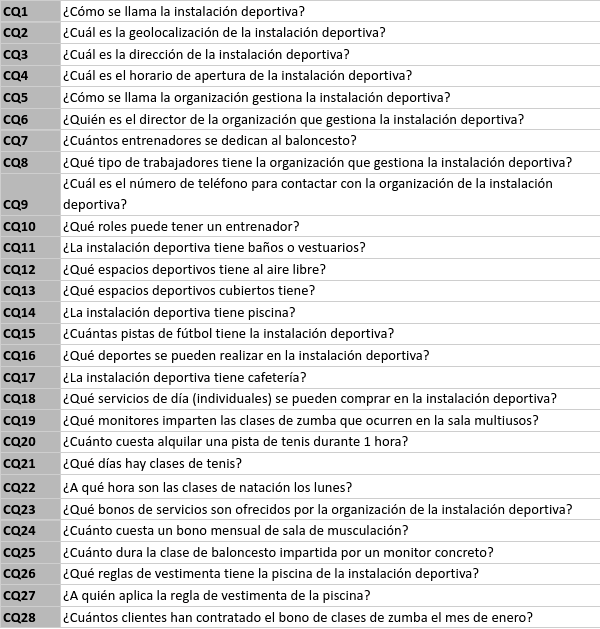
\includegraphics[width=0.9\textwidth]{include/preguntas_competencia.png}
		\caption{Preguntas de competencia}
	\end{figure}
	
	\subsection{Glosario de términos}
	
	Tras realizar las preguntas de competencia, hemos contado los sustantivos relevantes que se repetían, tanto en las preguntas para identificar clases y relaciones, como en las respuestas. 
	
	Cabe destacar que las preguntas se han contestado de manera muy genérica, sin concretar para una Instalación específica, de forma que los términos recogidos están un nivel por encima de ser instancias. Los resultados de algunos de los términos más relevanten se recogen en la siguiente figura: 

	\begin{figure}[H]
		\centering
		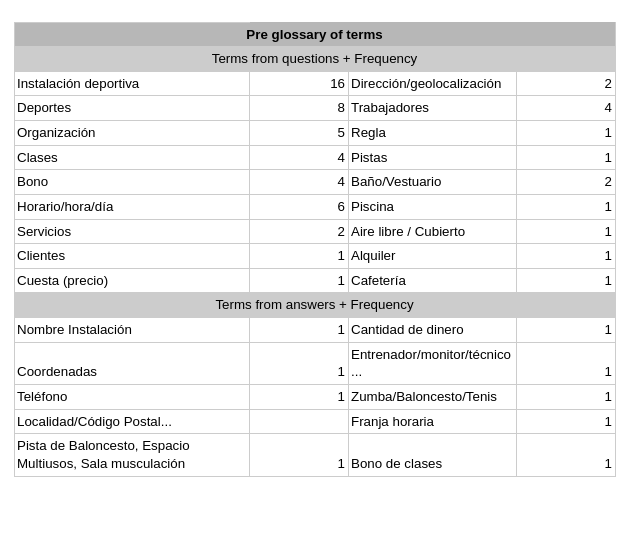
\includegraphics[width=0.9\textwidth]{include/terms.png}
		\caption{Glosario de términos}		
	\end{figure}
	
	\section{Planificación temporal de la ontología}
	% Ontology Schedule. You should identify the ontology life cycle model you use in your ontology development. Activities should come from the glossary of terms. Include a Gantt chart with the planned activities.
		
	El ciclo de vida utilizado en el diseño y desarrollo de esta ontología es el ciclo de vida incremental, pudiéndose considerarse como la primera iteración de un modelo ágil.
	
	Se decidió utilizar un ciclo de vida incremental debido a las características del proyecto, ya que la ontología no fue diseñada a partir de un set de datos proporcionados por el cliente, si no que se realizó el modelado a partir de las posibles necesidades de sus usarios. 
	
	La planificación temporal se puede dividir en varias secciones. Durante la planificación de la ontología se buscó el ámbito sobre el que realizar el trabajo, un tema sobre el que no existiesen ontologías ya diseñadas, y se definieron los requisitos planteando las preguntas de competencia. Se diseñó la ontología reutilizando los recursos útiles encontrados plasmándolos en el modelo conceptual. A continuación se creó la implementación del modelo y su evaluación. La redacción de este documento se puede considerar un ejercicio transversal.
	
	\begin{figure}[H]
		\centering
		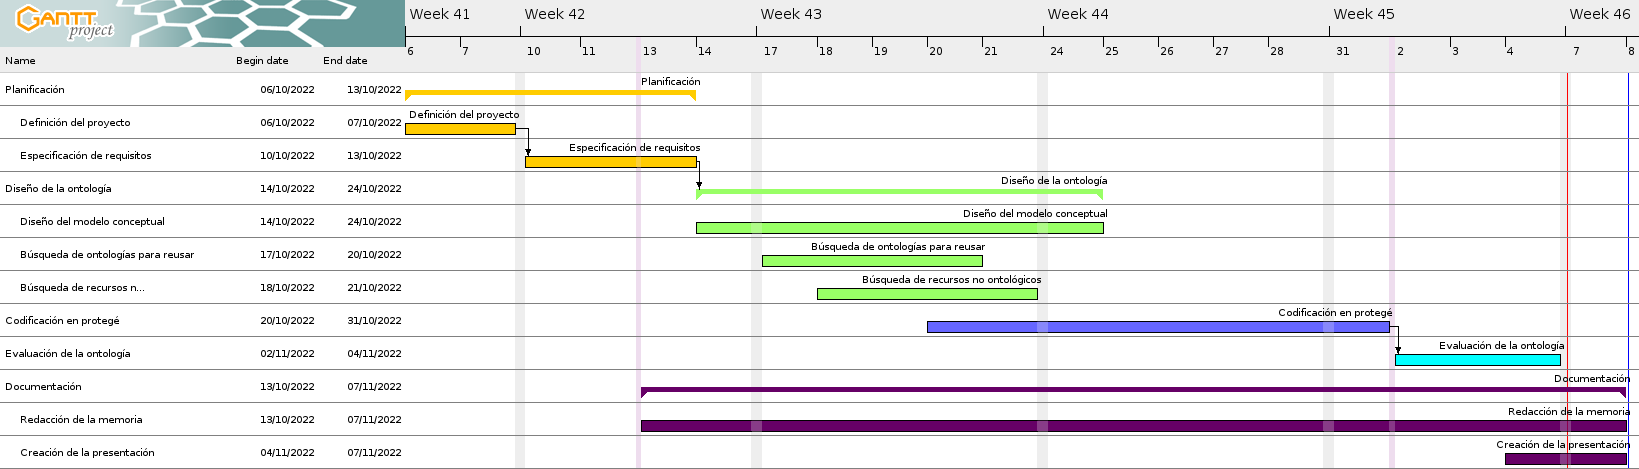
\includegraphics[width=\textwidth]{include/gantt_ontologia.png}
		\caption{Diagrama de Gantt de la planificación temporal seguida.}
	\end{figure}
	
	\section{Búsqueda de ontologías de alto nivel}
	% Search for existing top level and domain ontologies that you plan to reuse when building your ontology. Explain if you need to reuse the ontology as a whole or if you need some modules or statements. Explain in which repositories you made the search, ontologies found, their relevance to your work and the criteria being used for selecting or withdrawing some of them.
	
	Una vez identificados el glosario de términos mediante la especificación, y creado un modelo donde se relacionan las diferentes entidades, el siguiente paso es la formalización de la ontología. Para ello, hemos realizado una búsqueda de ontologías de alto nivel, detectando aquellas que cubren de manera total o parcial secciones de nuestro modelo para poder reutilizarlas.
	
	Las primeras ontologías que hemos identificado para nuestra ontología, fueron mencionadas a lo largo del curso:
	\begin{itemize}
		\item \textbf{Org.} La ontología org ha sido utilizada para representar la entidad de la organización que lleva la instalación deportiva. No hemos utilizado la ontología completa, solo los módulos que nos hacían falta para representar la organización, su localización y sus miembros. Esta ontología es ampliamente utilizada: en LOV, podemos ver que 37 ontologías reutilizan contenido de org.
		\item \textbf{Foaf.} Para poder representar a todas las personas que pertenecen a nuestro modelo (director, entrenadores, monitores, deportistas...) hemos utilizado foaf. A efectos prácticos, nos ha servido con importar la ontología org, ya que esta contenía las entidades foaf que nos hacían falta
		\item \textbf{Odrl.} La ontología ODRL permite modelar reglas y políticas. Se ha utilizado para representar las reglas de vestimenta en los espacios deportivos. Para ello, se ha utilizado únicamente parte de la ontología, en concreto las entidades que son necesarias para generar el patrón Norm, que describiremos más adelante.
		\item \textbf{Geo.} La ontología Geo se ha utilizado para poder expresar la geolocalización de la instalación mediante la entidad GeoPoint. Esta ontología no tiene propiedades, así que hemos tenido que crear una propiedad que relacione la instalación con el GeoPoint. 
		\item \textbf{Vcard.} Consiste en una ontología utilizada para representar la información que contiene una tarjeta de visita. En nuestro caso, hemos utilizado únicamente las entidades referentes a la dirección (Address) y nombre (OrganizationName).
		
	\end{itemize}
	Una vez identificadas estas ontologías de alto nivel, utilizamos el buscador de LOV (Linked Open Vocabularies) para buscar otras posibles ontologías que pudiéramos reutilizar. En concreto encontramos las siguientes:
	
	\begin{itemize}
		\item \textbf{Time.} La ontología time permite expresar tanto fechas como intervalos y duración de eventos. En nuestro caso, para expresar la fecha y la duración de los servicios hemos utilizado dos entidades diferentes.
		\item \textbf{Sport.} Esta ontología estaba disponible en el buscador, pero las URIs no llevaban a ninguna ontología, por lo que no pudimos reutilizarla. 
	\end{itemize}
	A la hora de importar todas estas ontologías en protegé, utilizamos LOV como método de búsqueda de las URIs, lo que facilitó la tarea. 
	
	\section{Recursos no ontológicos}
	%Search for non ontological resources and other terminologies that could be transformed into ontologies. Keep track of the URLs where you found them. For the selected resources, do not forget to justify why you have selected them. Check if you have Access rights for using them within your hands-on assigment.
	
	Una de las fuentes de información utilizadas para generar la ontología propuesta en este documento es el siguiente informe \cite{pdf-culturaydeporte}. A partir de este recurso no ontológico, mediante el uso de un T-Box se pudo realizar una modelización de la información descrita que representa la estructura taxonómica del documento en esta ontología de instalaciones deportivas. 
	
	El documento \cite{pdf-culturaydeporte} del Ministerio de Cultura y Deporte del Gobierno de España, contiene los  principales resultados del informe de explotación estadística del censo de instalaciones deportivas de 2005, así como las definiciones de las diferentes clases de instalaciones deportivas consideradas durante el censo.
	
	Al plasmar el conocimiento presente en este documento en el modelo de la ontología mediante un T-Box, se decidió mantener las clases intermedias presentes en el documento como parte de la ontología pese a que serán probablemente rara vez utilizadas para mantener la estructura del documento mencionado y facilitar la reutilización de este. 
	
	\begin{figure}[H]
		\centering
		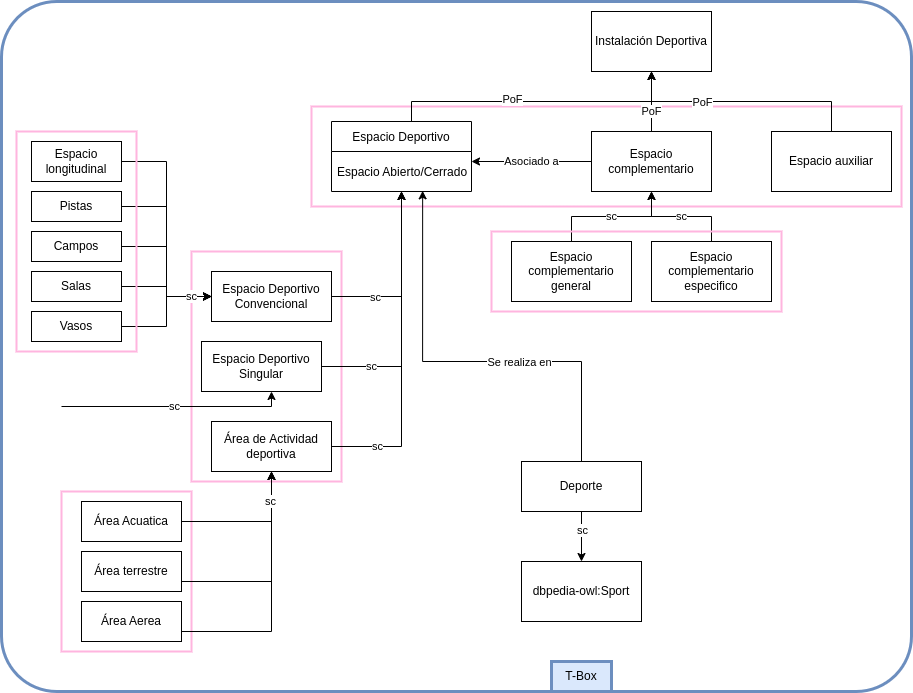
\includegraphics[width=0.7\textwidth]{include/tbox.png}
		\caption{Sección correspondiente a los recursos no ontológicos en la ontología.}
	\end{figure}
	
	Es importante señalar que la estructura taxonómica del documento descrito exige desambiguar entre las relaciones "sub-clase de" (\textit{sc} en el diagrama) y "parte de" (\textit{PoF} en el diagrama).
	
	\section{Patrones en la ontología}
	% Search for some ontology design patterns in the ontology design pattern portal that could be reused in your development.
	
	Para facilitar el diseño de los servicios ofrecidos por la organización en una instalación deportiva, se reutilizó el patrón de una relación N-aria según lo visto en clase. Este patrón se utiliza para representar una relación N-aria en el que todos los elementos tienen la misma importancia. Para representar esta relación N-aria se crea una clase, en nuestra ontología la clase \textit{ServicioOfrecido}, a la que asociar todos los atributos de la relación.
	
	\begin{figure}[H]
		\centering
		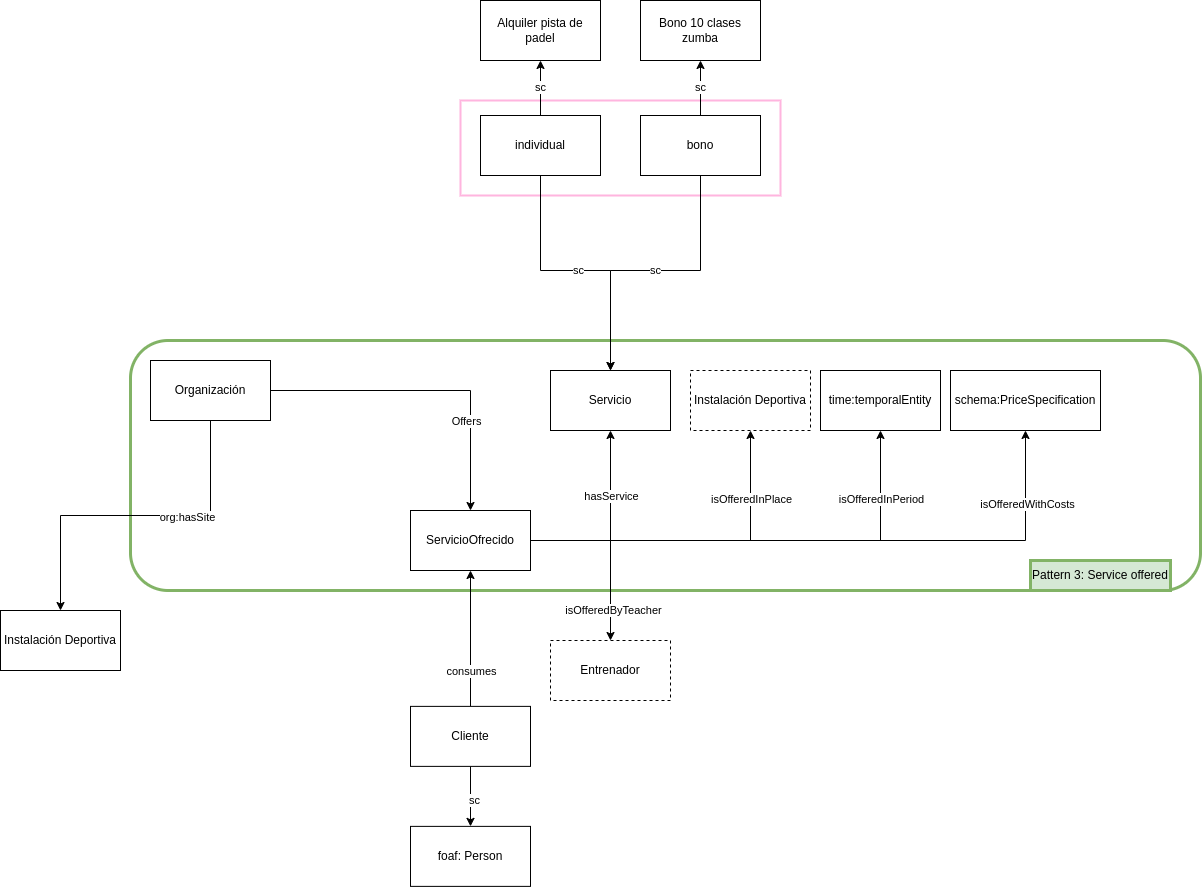
\includegraphics[width=0.5\textwidth]{include/patron.png}
		\caption{Sección correspondiente a los patrones utilizados en el diseño de la ontología.}
	\end{figure}
	
	
	\section{Modelo conceptual}
	% Build a conceptual model that integrates outcomes from the previous sections (c,d,e). This is the most important part of the work you are doing. Try to use:
	%  	i. Top level ontologies and other well-known ontologies. Classify in the pyramid of ontologies (figure use vs reuse) each of the ontologies that you reuse.
	%   ii. Transform each non-ontology resource into an ontology by using the T-box, A-Box or Population.
	%   iii. Select some Ontology Design Patterns (events, sequence, etc.)
	%   iv. Build the conceptual model of your ontology by integrating the above sources. The conceptual model should have at least 40 concepts, several subclass-of relations, disjoint, part-of (if needed), and ad-hoc relations.
	
	\section{Clases Multilingües}
	
	\section{Implementación de la ontología con OWL}
	% Implement the ontology in an ontology development tool, or other ontology editor, using OWL as ontology language
	
	Una vez identificados el glosario de términos mediante la especificación, y hemos conceptualizado un modelo donde se relacionan las diferentes entidades, el siguiente paso, la formalización de la ontología. Para ello, hemos realizado una búsqueda de ontologías de alto nivel, de forma que si alguna de ellas cubre toda o parte de alguna de nuestras entidades, podamos \textbf{reutilizarla.
	}.\\
	Las primeras ontologías que hemos identificado para nuestra ontología, fueron mencionadas a lo largo del curso:
	\begin{itemize}
		\item \textbf{Org:}La ontología org ha sido utilizada para representar la entidad de la organización que lleva la instalación deportiva. No hemos utilizado la ontología completa, solo los módulos que nos hacían falta para representar la organización, su localización y sus miembros. Esta ontología es ampliamente utilizada: en LOV, podemos ver que 37 ontologías reutilizan contenido de org.
		\item \textbf{Foaf: }Para poder representar a todas las personas que pertenecen a nuestro modelo (director, entrenadores, monitores, deportistas...) hemos utilizado foaf. A efectos prácticos, nos ha servido con importar la ontología org, ya que esta contenía las entidades foaf que nos hacían falta
		\item \textbf{Odrl:} La ontología ODRL permite modelar reglas y políticas. Se ha utilizado para representar las reglas de vestimenta en los espacios deportivos. Para ello, se ha utilizado únicamente parte de la ontología, en concreto las entidades que son necesarias para generar el patrón Norm, que describiremos más adelante.
		\item \textbf{Geo:} La ontología Geo se ha utilizado para poder expresar la geolocalización de la instalación mediante la entidad GeoPoint. Esta ontología no tiene propiedades, así que hemos tenido que crear una propiedad que relacione la instalación con el GeoPoint. 
		\item \textbf{Vcard: }Consiste en una ontología utilizada para representar la información que contiene una tarjeta de visita. En nuestro caso, hemos utilizado únicamente las entidades referentes a la dirección (Address) y nombre (OrganizationName).
		
	\end{itemize}
	Una vez identificadas estas ontologías de alto nivel, utilizamos el buscador de LOV (Linked Open Vocabularies) para buscar otras posibles ontologías que pudieramos reutilizar. En concreto encontramos las siguientes:
	
	\begin{itemize}
		\item \textbf{Time:} La ontología time permite expresar tanto fechas como intervalos y duración de eventos. En nuestro caso, para expresar la fecha y la duración de los servicios hemos utilizado dos entidades diferentes.
		\item \textbf{Sport:} Esta ontología estaba disponible en el buscador, pero las URIs no llevaban a ninguna ontología, por lo que no pudimos reutilizarla. 
	\end{itemize}
	A la hora de importar todas estas ontologías en protegé, utilizamos LOV como métode de búsqueda de las URIs, lo que facilito la tarea. 
	Como se ha especificado en los requisitos, la onotlogía estará implementada en OWL. Para eso, hemos utilziado protégé, un editor de ontologías open source. \\
	
	El primer paso que hemos hecho ha sido incluir todas las clases de la ontología que hemos creado mediante el T-Box. Después, hemos reutilizado de las ontologías nombradas en el apartado 5 todas las clases que nos hacían falta. Para ello, hemos importado las ontologías con su URI y movido los axiomas necesarios a nuestra ontología.
	
	En general, la metodología para importar las ontologías ha sido idéntica para todas: primero hemos importando la ontología al completo con su uri, moviendo los axiomas que necesitábamos, y después hemos eliminando el resto. La única excepción ha sido la ontología Time. 
	
	Hemos importado la ontología Time de forma completa, ya que utilizábamos la totalidad de sus entidades. Al importar la ontología, nos hemos dado cuenta de que muchas de las propiedades estaban incompletas: les faltaba el rango o el dominio. Hemos optado por mantenerla como estaba, ya que muchos de estos problemas se debían a términos deprecados, y no hemos encontrado una versión más reciente de la ontología.
	
	Una vez importadas las clases necesarias, hemos definido aquellas que nos hacían falta para completar nuestro modelo, que no se encontraban ni en el T-Box ni en las ontologías de alto nivel, como puede ser por ejemplo la clase Monitor, Entrenador, Pista de Baloncesto... A continuación se muestra una imagen de la jerarquía de las clases.
	
	\begin{figure}[H]
		
		\centering
		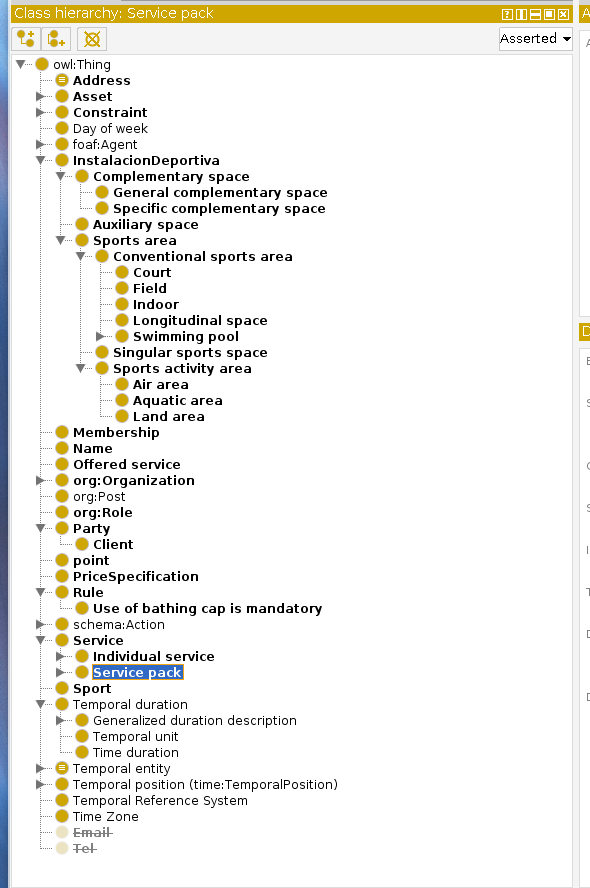
\includegraphics[width=0.6\textwidth]{include/classes.png}
		\caption{Classes}
	\end{figure}
	
	Este mismo procedimiento lo hemos realizado para los Object Properties. En este caso, a demás de importar los necesarios de las diferentes ontologías y crear los que necesitabamos, hemos definido las propiedades de cada propiedad. 
	
	Hemos tenido cierta dificultad a la hora de crear la propiedad Part Of, ya que tiene varios dominios para un único rango (tanto los espacios deportivos, como los complementarios y auxiliares son part of de una instalación deportiva). Para evitar interferencias, hemos incluido los diferentes dominios con la condición OR. 
	
	En la imagen a continuación se pueden ver los diferentes Object Properties de la ontología.
	
	\begin{figure}[H]
		\centering
		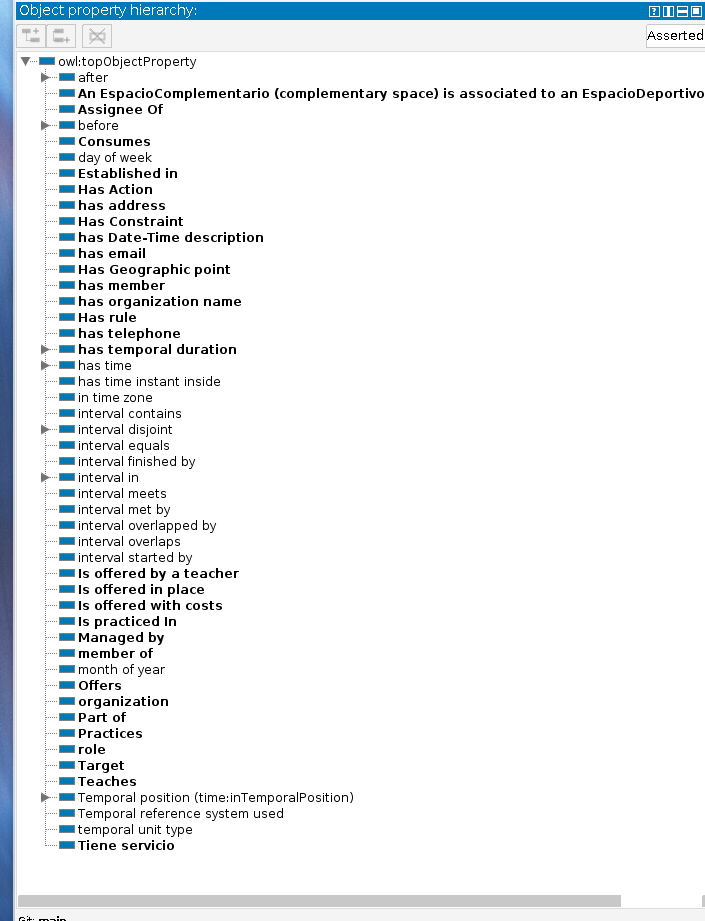
\includegraphics[width=0.6\textwidth]{include/object.png}
		\caption{Object Properties}
	\end{figure}
	
	De forma similar hemos añadido los Data Properties. Estos en lugar de apuntar a una entidad, apuntan a un literal, por lo que hemos tenido que especificar los tipos de datos para literales como la divisa, el precio... Un caso particular ha sido la propiedad hasCeiling (tiene techo), para definir los Espacios Deportivos. En este caso el literal era un booleano. A continuación se muestran las diferentes Data Properties. 
	\begin{figure}[H]
		\centering
		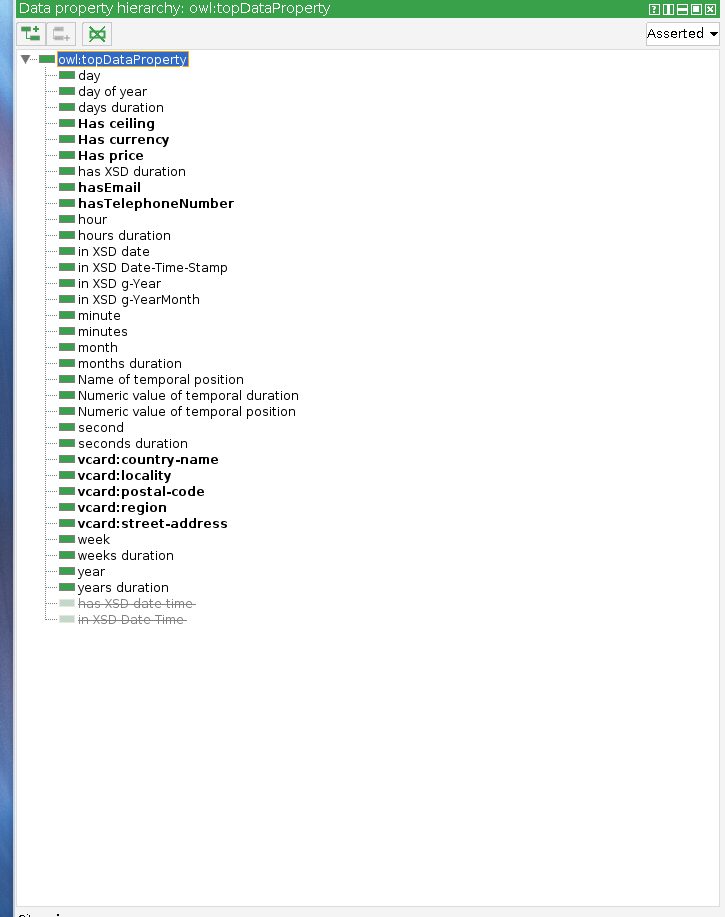
\includegraphics[width=0.6\textwidth]{include/data.png}
		\caption{Data Properties}
	\end{figure}
	
	Finalmente, hemos completado las labels y comentarios de aquellas entidades que no han sido directamente importadas, asegurandonos de que estaban disponibles tanto en inglés como español. \\
	
	Una vez finalizada la implementación de la ontología, la hemos exportado como RDF para poder evaluarla con OOPS!
	
	\section{Evaluación de la ontología con OOPS!}
	% Evaluate the ontology with OOPS! and include in your report the pitfalls found. It is highly advisable to combine this evaluation with other ontology evaluation techniques.
	% Improve your ontology (conceptual model and implementation) taking into account the suggestions given by OOPS!. Iterate in these steps until the ontology pass most of the OOPS! recommedations.
	La ontología diseñada se ha evaluado utilizando la herrramienta OntOlogy Pitfall Scanner! (OOPS!)\cite{oops}, que identifica errores en la ontología dividiéndolos en críticos, importantes y menores, de acuerdo a una batería errores comunes.
	
	\subsection{Mejoras implementadas tras la sugerencia de OOPS!}
	
	Tras la primera iteración de la evaluación con OOPS!, la herramienta destacó los siguientes problemas críticos:
	
	\begin{itemize}
		\item \textbf{P19:} Propiedades con múltiples rangos o dominios.
		
		Una de las relaciones definidas tenía más de un dominio, habiendo escrito en Protegé accidentalmente \textit{and} en lugar de \textit{or} en el dominio. Este error fue solucionado.
		\item \textbf{P29:} Relaciones transitivas mal definidas.
		
		Las relaciones \textit{partOf}, \textit{hasService}, \textit{managed\_by} y \textit{constraint} estaban definidas como transitivas, teniendo rangos y dominios distintos. Por definición una propiedad transitiva debe tener el mismo rango y dominio. Este error fue solucionado.
	\end{itemize}
	
	Gracias a los errores destacados por OOPS! se pudieron solucionar todos los errores críticos y varios errores clasificados como importantes. Se decidió no solucionar los errores no críticos de las ontologías importadas debido a las restricciones temporales sobre la entrega del trabajo.
	
	\subsection{Resultados finales de la evaluación}
	
	Tras aplicar las correcciones sobre las sugerencias de OOPS! la ontología tiene \hl{xx} errores importantes y \hl{xx} errores menores.
	Los resultados completos de esta evaluación se pueden encontrar en el Anexo.
	
	\section{Documentación de la ontología}
	% Document the ontology with Widoco and use Ontoology if required
		
	\cite{widoco}
	
	%\includepdf[pages=-]{include/documentation-widoco.pdf}
	
	\section{Conclusiones}
	
	
\newpage
	\section*{Bibliografía}
	\addcontentsline{toc}{section}{Bibliografía}
	\bibliography{include/references}
	\bibliographystyle{IEEEtran}
	
	\newpage
	\section*{Anexos}
	\begin{figure}[H]
		\centering
		%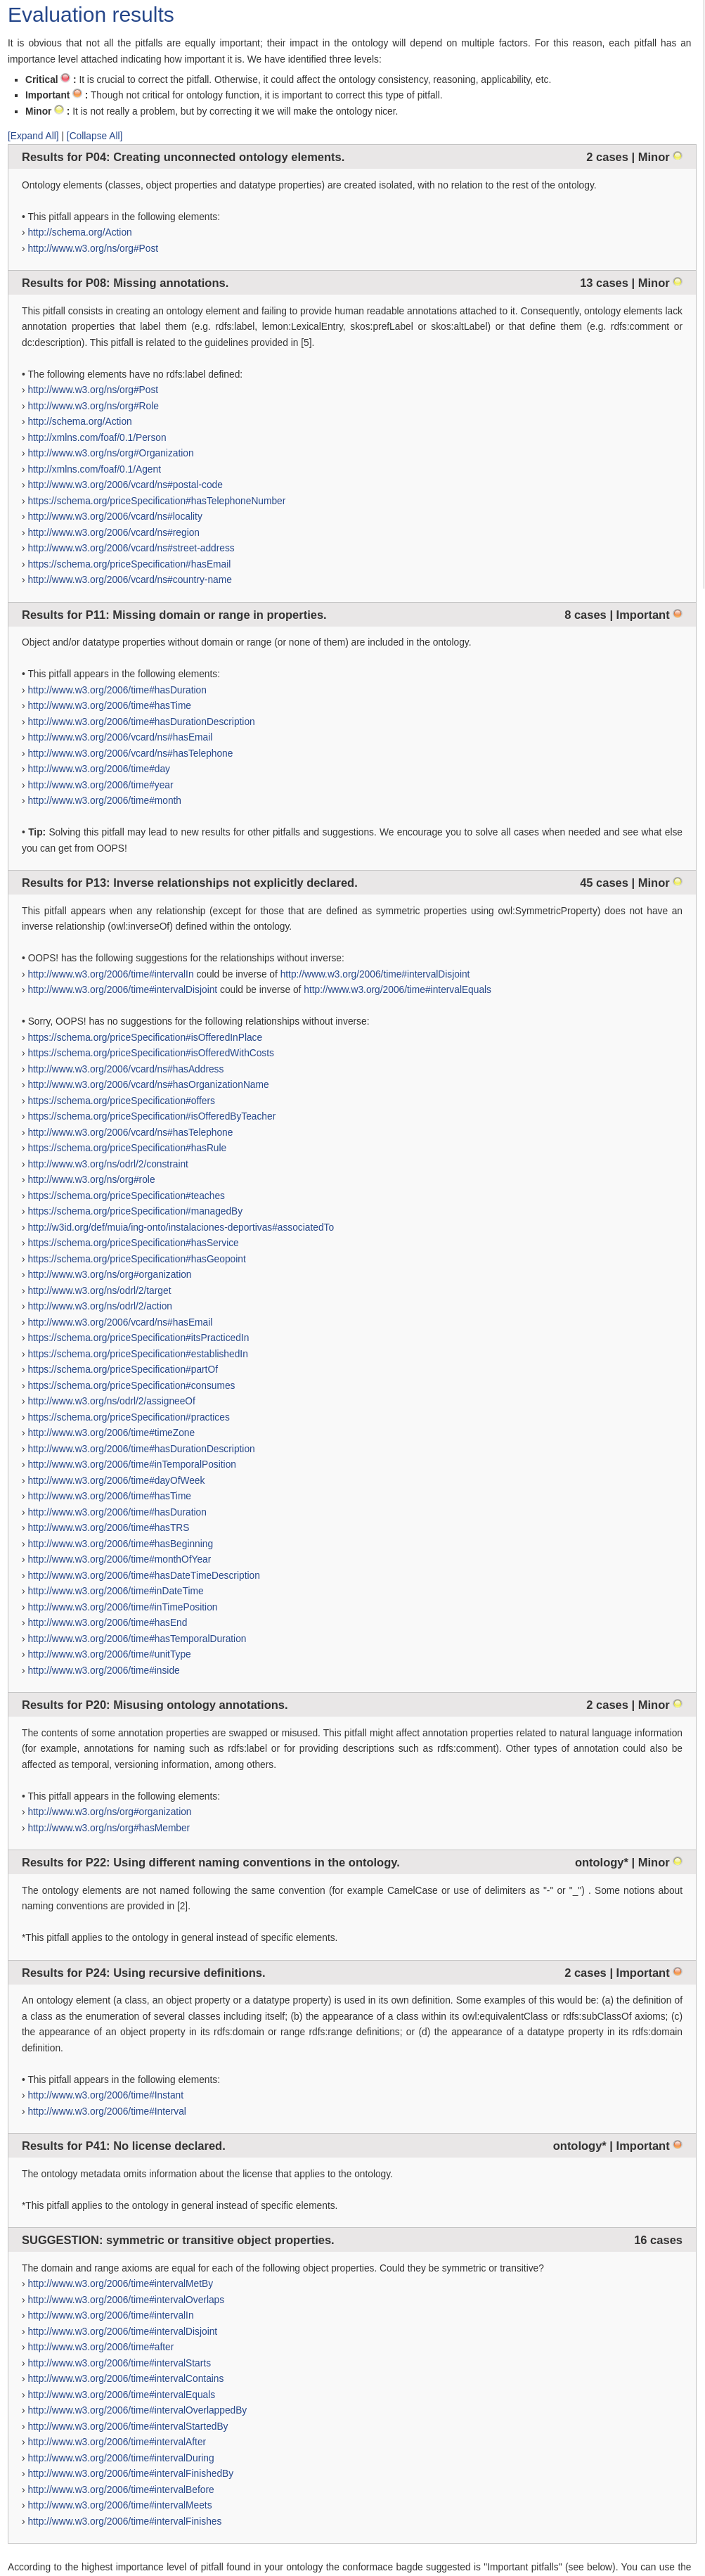
\includegraphics[height=\textheight]{include/eval_final_oops.png}
		\caption{Resultados finales de la evaluación con OOPS!}
	\end{figure}

\end{document}